\documentclass[journal,twoside,web]{ieeecolor}
\usepackage{jsen}
\usepackage{cite}
\usepackage{amsmath,amssymb,amsfonts}
\usepackage{algorithmic}
\usepackage{graphicx}
\usepackage{textcomp}
\usepackage{wrapfig}
\def\BibTeX{{\rm B\kern-.05em{\sc i\kern-.025em b}\kern-.08em
    T\kern-.1667em\lower.7ex\hbox{E}\kern-.125emX}}
\markboth{Spring 2020}
{Pathan Faisal Khan: Big Data Analytics}
\begin{document}
\title{Graph Analytics for Big Data Analytics}
\author{Pathan Faisal Khan
\thanks{Under the supervision of Dr. Shagufta Henna, Letterkenny Institute of Technology, Letterkenny, CO. Donegal}
}

\IEEEtitleabstractindextext{
\begin{abstract}
The term big data has quite a significance. It deals with data of huge volumes. This data might be and might not be structured and if structured it might be and might not be of the same data structure. So for different data structures, different types of analytical approaches have to be defined. This paper specifically deals with the analysis of graph data in big data. The focus of this paper will be on distributed computing algorithms. Different types of graph analysis are covered in this paper. This paper has reviewed path analysis which is used for determining a path with minimal distance amongst two nodes, connectivity analysis which is used for analyzing weaknesses in the network, community analysis used to focus on the interactions between nodes, and centrality analysis method which is used to find the relevance between each node. Along with these techniques, the paper has investigated Graph Neural Networks. Because of challenges in GNN, many methods were proposed recently\cite{33}.

\end{abstract}

\begin{IEEEkeywords}
Big Data Analytics, Centrality Analysis, Community Analysis, Connectivity Analysis, Graph Analytics, Graph Neural Network, Path Analysis
\end{IEEEkeywords}}

\maketitle

\section{Introduction}
\label{sec:introduction}
\IEEEPARstart{W}{ith} the introduction of the internet in the 90s, there has been tremendous innovation in the tech industry. This changed the way organizations, businesses, governments function. It even changed the lifestyle of the people. Major contributions to the tech space were not until the early 2000s due to innovations in computational power and during this period, the volume of data generated with the introduction of social media and other services for the masses has risen a lot. Data is being created every second of the data. In 2013, Instagram users shared 3600 photos every minute, while in 2019, the number of photos shared every minute reached 46,740. The world internet population has increased from 2.5 billion to 3.7 billion~\cite{1}. It is estimated that by 2020, 40 trillion GB of data would be generated~\cite{2} which means internet user generates nearly 2500000 terabytes of data every day~\cite{1}. Most of the data being generated is contributed by social media on which an average user spends 33\% of his/her online time. This is why in 2019, there are 2.3 billion users active on Facebook~\cite{3}.

Because of this vast amount of data, there was a need to develop more efficient and cost-effective data storage. This led to the introduction of the term Big Data in early 2005~\cite{4}. Big data is the type of data that has a high variety, large volume, high velocity, greater veracity, and extreme value also it is continuously growing on a large scale. These characteristics of the big data are referred to as the 5Vs. It will not be a surprise that the data is unstructured as it is being collected from multiple sources. Big data can be comprised of logs of the traffic coming in on a website, messages generated on a social media site, attributes of mouse clicks, details of products stored on an e-commerce website, medical data of a hospital, bank transactions, satellite data, and many other sources which generate data.

Since generating data is an easier task than getting useful insights out of it, there was a need to emphasize on its analysis. But because of the sheer volume of high dimensional, unstructured, and highly inconsistent data, running traditional methods for analysis might miss out on the hidden structures of the data. Thus, there was a need to devise powerful algorithms and provide high computational powers that can solve these problems. Due to the introduction of cloud computing and its scalable nature, researchers were able to develop algorithms to mine and make out meaningful insights from this data. With the right analysis methods, it can yield greater insights leading to stronger and strategic decisions. Using big data analysis, Netflix manages to easily save \$1 billion every year~\cite{5}. Wikibon, an organization sharing tech-related knowledge, has estimated the market worth of big data analytics to a whopping \$49 billion for the year 2019~\cite{6}.



This paper will discuss some graph analysis methods used on big data in Section \ref{sec:lit_review}. A comparison will then be done on some of these techniques in Section \ref{sec:discussion}. Also, Graph Neural Network will be briefly explored along with other graph analytic techniques in \ref{sec:gnn}. The paper will finally conclude with the observations from this report in Section \ref{sec:conclusion}.

\section{Graph Analytics}
\label{sec:lit_review}
Often data generated have relations among themselves. This data can be structured or unstructured or a mix of both. Since it is not feasible to understand these relations using the traditional big data analytics techniques, a better model had to be devised. A graph model was proposed to connect the data. Graphs are effective for analyzing, making recommendation systems, and mining social networks. Due to the flexibility of this model it allows large quantities of information from many sources to be quickly absorbed and linked in ways that addressed the limitations in the source structures. A good way of representing the graph model is connections of a social media account; it represents a graphical structure with connections (edges) formed between different accounts (nodes/entities). This model enabled analyzing relationships and deducing interesting patterns between accounts (entities) in the structure. Graph analytics is a term used to define these methods of analysis. It is defined as an alternative to the conventional data warehouse model as a system for allowing analysts to check structured and unstructured data from different sources. Some business use cases of graph analytics include healthcare quality analysis, cybersecurity, and correlation findings.

\subsection{Path Analysis}
Path analysis algorithms are used for exploring a graph that may either lead to the discovery of new or optimal paths. A path may be decided as an optimal path on basis of the number of hops required to traverse, weights of visited nodes, avoiding/including specific nodes/paths or in some cases based on an optimization function. One of the most common use cases is getting the shortest path using Google Maps directions. Some other applications include but not limited to are customer behavior analysis on an e-commerce website and re-routing in a network to fix problems with network capacity. This paper is going to cover briefly some path analysis algorithms in the following sections.

\subsubsection{Parallel Breadth-First Search}
To understand parallel breadth-first search, serial or conventional breadth-first search (BFS) will be explored first. Since the paper is dealing with graph-based analysis methods, BFS will be covered for graph implementation rather than tree implementation. The difference between both implementations will also be covered in this section.

The BFS algorithm starts at an arbitrary node in the graph and travels to all nodes at the current level $n$ and then proceeds to the next level $n + 1$ of the graph. The following figure \ref{fig1} shows the order of expansion/exploration of nodes. This example shows a graph without loops in it. This is the major difference between a graph and a tree; a graph may have loops in it, while a tree does not have loops. Hence, to avoid the loops, BFS implementation of a graph is different as it requires a mechanism to track visited nodes to avoid unnecessary infinite loops.

\begin{figure}[!h]
    \centerline{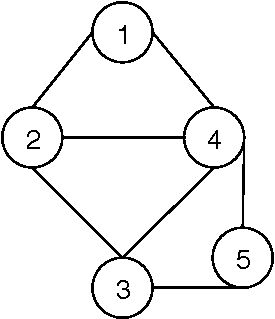
\includegraphics[scale=1]{figures/bfs.pdf}}
    \caption{The numbers depict the order of traversal of nodes in a BFS implementation}
    \label{fig1}
\end{figure}

The problem with serial BFS is that time and memory consumption depends on the number of branches and the depth of the graph. In worst case, for a graph with ${b}$ branches and ${l}$ levels, time and space complexity is then given by O($b^l$). Since we are dealing with big data analysis where data is huge, it will consume a lot of time.

To solve this issue with BFS, the concept of parallelism was introduced. Parallel computing distributes the load to multiple processors hence taking of load from a single process and distributing it to others to reduce the overhead. The parallel version of BFS can be done using two approaches either using shared memory or by using distributed memory. The shared memory implementation of BFS generates Breadth-First Spanning Trees (BFSTs) of a given graph G with $n$ nodes. The time complexity of this step is given by O($log(d).log(n)$) where $d$ is the diameter of G which is far more better than serial BFS with time complexity O($b^d$). The number of processors used for this process depends on the number of nodes; the time complexity is defined by O($n^3$) \cite{36}. If the graph is undirected, the algorithm will generate $n$ BFSTs.

In the distributed memory version of BFS, each process has its memory and they have to share messages amongst each other to share their data. Since there is an overhead of communication in this approach, shared memory BFS will provide higher bandwidth with low latency \cite{37}.

\subsubsection{Parallel Depth-First Search}
Parallel depth-first search also deals with parallelism as discussed in the previous section. To understand this, its necessary to go through serial depth-first search (DFS).

The DFS algorithm starts at an arbitrary node and travels deep into a path before coming back a step and exploring the next path. This algorithm is used on hierarchical data. Since the algorithm might face issues with infinite loops due to the fact we are traversing on a graph, similarly to BFS, DFS for graphs also have to be implemented with a mechanism to store visited nodes. The time complexity of DFS is similar to BFS, O($b^d$) while the space complexity is O($d$).

Serial DFS also faces the same problem as serial BFS, that is it will also consume a lot of time for big data analysis. So to avoid this, parallel DFS was proposed. To parallelize DFS, the graph is split among different processors. Each processor performs its task independently until it finishes it after which the processor requests an unfinished section of the graph from other processors. Some of the models of implementation of parallel DFS include shared memory models, boolean circuits, and parallel comparison trees\cite{38}.  

There are many implementations of parallel DFS and most of them showed logarithmic running time\cite{38}. Logarithmic running time is much more efficient than an exponential running time which is showed by a serial DFS.

\subsubsection{Single-Source Shortest Path}
Single-Source Shortest Path (SSSP) evaluates the shortest path from a given node to other nodes of a weighted digraph. It is also called as Bellman-Ford or Bellman-Ford-Moore algorithm\cite{41}. It was first proposed by Shimbel\cite{42} in 1955.

SSSP is capable of computing shortest path on graphs with "negative cycle" which makes it different from other shortest path algorithms. The algorithm works in bottom-up approach. It calculates first the shortest distance with at max one edge in a path, then it will consider edges with max two edges in the path and so on. It basically overestimates first the length of the path then reduces those estimations by finding shorter paths. 

\begin{figure}[!h]
    \centerline{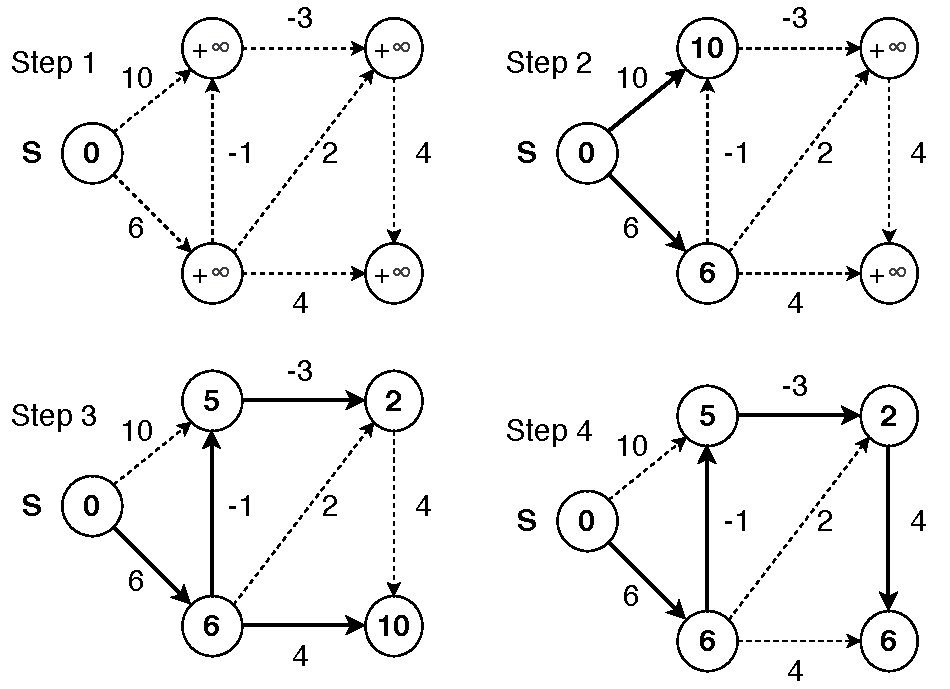
\includegraphics[scale=0.5]{figures/sssp.pdf}}
    \caption{Working of the SSSP algorithm on a "negative cycle" directed graph with 5 nodes}
    \label{fig2}
\end{figure}

In the above figure \ref{fig2}, shortest path of a graph is computed step-by-step using SSSP algorithm. Path costs are given. In step 1, all the nodes except start is initialized with positive infinity. Second step starts from the start node and traverses to all its neighbors. As the algorithm moves to its neighbors, path cost is assigned to the weights of the visited node. Now, in step 3, it can be noted that the node with weight 10 is replaced by 5 and the path from start to it is removed. The algorithm has computed a shortest path (path with least cost) from an alternate route even though it involves visiting one node before reaching to destination. This way, it computes and replaces weights as it proceeds to move through the graph. In step 4, we have the final path which costs just 6 to traverse through all the 5 nodes.

The time complexity of SSSP is given by O($V*E$) while the space complexity is O($V$) where $V$ denotes vertices and $E$ is edges of a graph. It is used for detecting link failures in a network and come up with new links or routes in no time.

\subsubsection{All-Pairs Shortest Path}
To understand All-Pairs Shortest Path (APSP) algorithm, the problem should be discussed first. APSP problem is for finding minimum distance between every vertices of a particular edge. The graph should be directed with weights. To solve this APSP problem, multiple variants of APSP algorithms were proposed\cite{43, 44, 45, 46}. This paper will first look into Floyd-Warshall algorithm which is quite popular amongst other APSP algorithms. Unlike SSSP, this algorithm does not work on "negative cycles" graph however, it can work on both directed and undirected graphs.

The output of this algorithm is a matrix representing the shortest distance from a node to other nodes. When a node is unreachable to an another node, the algorithm returns infinity which signifies no path can be formed. The figure shown below  



The time complexity of this algorithm is O($n^3$) where $n$ is number of vertices and space complexity is given by O($n^2$). Some common use cases of APSP algorithm are


\subsubsection{Minimum Weight Spanning Tree}
Minimum Weight Spanning Tree (MST) is applied on a tree where a path needs to be traced with minimum weight among all nodes. MST is used mostly to make clusters in a graph. K-Means is used along with MST to find clusters. MST was first developed by Borůvka in 1926\cite{47}. The most famous known adoption of Borůvka's algorithm was done by Jarnik in 1930\cite{48} which is sometimes called as Prim's algorithm as he rediscovered and republished it a few years later\cite{49}. Similar to SSSP, Jarnik's algorithm can be used on "negative cycle" graphs.

\begin{figure}[!h]
    \centerline{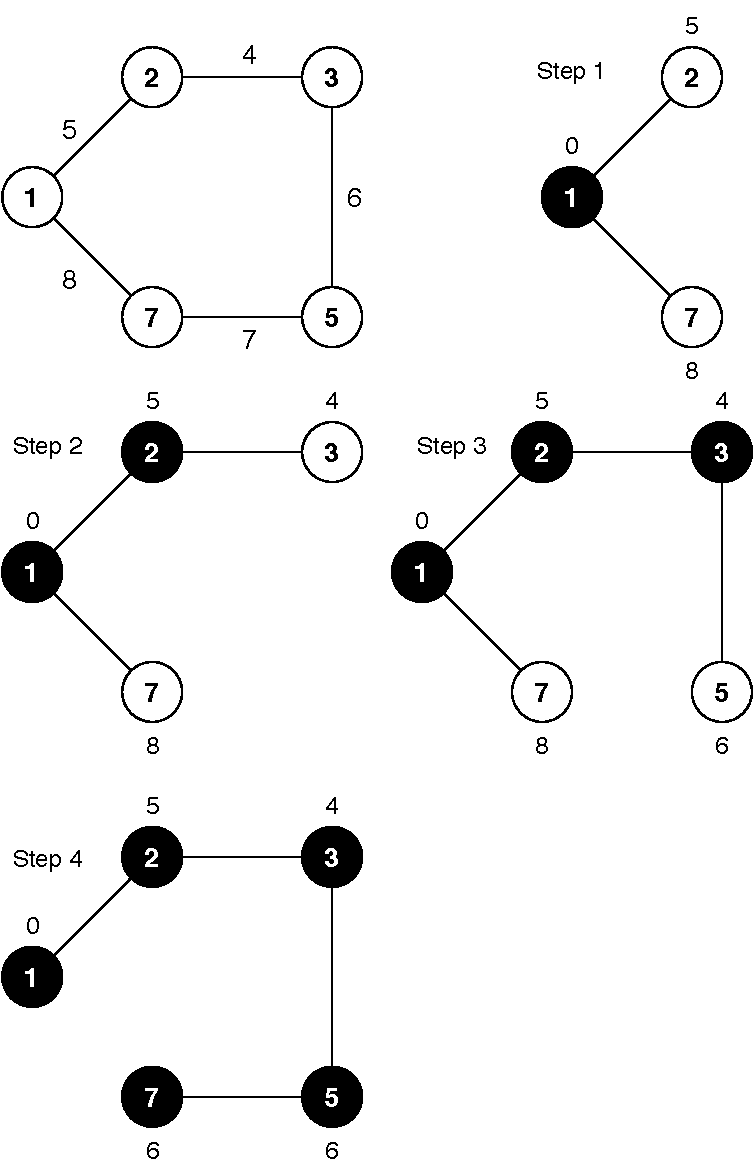
\includegraphics[scale=0.55]{figures/mst.pdf}}
    \caption{Step wise working of MST on a graph}
    \label{fig3}
\end{figure}

In above figure \ref{fig3}, MST is shown in action based on Jarnik's algorithm. In step 1, node 1 is picked up and its neighbors are assigned the path cost as a key-value pair. Node 1 is added to a list, hence darkened. In step 2, the lowest key-value pair among 7 and 2 is picked up, 2 is the lowest. Its neighbors is then assigned the weight as a key-value pair and 2 is added to the list. Similarly, in step 3 also 5 is assigned its weight. The algorithm will repeat this process until all nodes are added to the list. Now the order in which the nodes are picked up is our the path of the tree. It is noticed that individual node pair paths are considered rather than the whole tree while formulating the path.

Time complexity of this algorithm is O($v^2$) where $v$ is the number of vertices. This algorithm is used for analysing correlations between nodes in a graph. MST has been implemented to minimize commute cost in Papua New Guinea\cite{13} and for investigating molecular structure of Hepatitis C\cite{50}.

\subsubsection{Random Walk}
Random walk algorithm is a basic algorithm applied on analysing huge graphs. The algorithm starts at a node, randomly chooses a node to move to and then moves on to another randomly choosen node. The algorithm does this until it walks over all nodes in the graph. It maintains a list of visited nodes. This algorithm can be applied only on directed and unweighted graphs. Time complexity is given by O($\sqrt{n}\log(n)$) where $n$ is the population size.

Random walk has been used to analyse behvaiors; to analyse a pattern was invloved or it is random. It has been used in biology to understand biological processes\cite{51} and also been used to analyse stock market\cite{52}. Mostly random walk is used in conjugation with other algorithms\cite{53} or to improve training of machine learning algorithms\cite{54}. It is used as a clustering algorithm generally on graph data.

\subsection{Connectivity Analysis}
Connectivity analysis helps in identifying the strength of connections/vertices between two nodes in a graph. It is most commonly used for analyzing weaknesses in a graph network. Before diving into the algorithms, its important to understand how the strength of a connection is defined in a graph.

\subsubsection{Strongly Connected Components}
\label{sec:scc}
A component comprises two or more nodes connected. A concept of Strongly Connected Components (SCCs)\cite{39} is used. A component is said to be strongly connected when a given pair of nodes in the component has connections with each other.

\begin{figure}[!h]
    \centerline{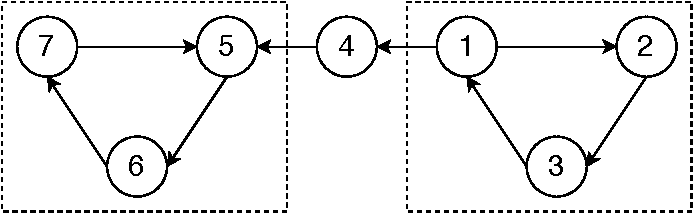
\includegraphics[scale=0.75]{figures/scc.pdf}}
    \caption{The graph shown has two SCCs with one node connecting both of them}
    \label{fig4}
\end{figure}

In the above figure \ref{fig4}, there are two SCCs, one with {$1, 2, 3$} nodes and the other with {$7, 5, 6$} nodes connected with node $4$. As can be seen that $1$ is connected with $2$ and $2$ is connected with $3$ which is then connected with $1$, thus it is said that both of these components are strongly connected.

SCCs help in forming clusters in a graph. With the help of such clusters, analysis can be performed in the network. Some use cases of connectivity analysis includes social network and internet network analysis. Now the problem lies in finding out such SCCs. DFS and BFS help find such components. Kosaraju devised an algorithm which in linear time helped in finding out SCCs\cite{40}. This paper will cover Kosaraju's algorithm's modification on BFS and DFS.

\subsubsection{Kosaraju's BFS and DFS}
Kosaraju's original proposed algorithms were based on DFS and some implementations exist of it on BFS. The DFS implementation does a simple trick by performing DFS two times on the same graph. Taking figure \ref{fig4} as an example, the algorithm will perform the first DFS on the graph. It will reverse the directions in the graph and start at $7$, explore in the order $7-6-5-4-1-3-2$. Now the node which finished first or visited at the end will be assigned the finishing position starting from 1. The nodes will be renamed with their corresponding positions as shown below in figure \ref{fig5}. 

\begin{figure}[!h]
    \centerline{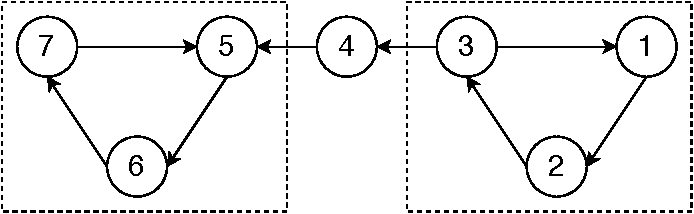
\includegraphics[scale=0.75]{figures/scc2.pdf}}
    \caption{Nodes renamed with their position after the first DFS}
    \label{fig5}
\end{figure}

Now second DFS will be performed and as $7$ was the start node previously, this time also it will start from $7$. The order will be then $7-6-5$ which is our first SCC and then starting DFS from $3$, the order will be $3-1-2$ which is our second SCC. Thus, the algorithm pointed out two SCCs in the graph. Time complexity of Kosaraju’s DFS is O($n + e$) where $n$ is nodes of the graph and $e$ is edges.

Kosarju's BFS algorithm also works in the same way; it performs BFS twice instead of DFS.

\subsection{Community Analysis}
A community in a graph network is defined by a group of nodes that have dense connections amongst themselves and sparse connections with the other group of nodes. Community analysis points out interactions between nodes. It is used for clustering nodes with similar attributes. This analysis also helps in analyzing how nodes are clustered or partitioned. The strength of a particular group can also be determined by this analysis. Community analysis is used in identifying proteins involved in a biochemical process, recommendations for a group of people, and evaluating social networks. 

Strongly connected components has been discussed in the previous section \ref{sec:scc} which is a part of community analysis. Weakly connected components also helps in defining structure of the graph by analysisng nodes which are loosely connected in a graph.

\subsubsection{Label Propagation}
Raghavan et al. proposed this algorithm back in 2007\cite{16}. The algorithm worked on exploring communities in a graph network. 

The algorithm functions in the following way. Consider a node $n$ with neighbors $n1, n2, n3$ and so on also every node has a tag identifying them with which community they are a member of. Therefore, $n$ will identify its community based on its neighbors' communities. So the algorithm starts with assigning a unique tag on all nodes present in the graph; this part of the algorithm suggests that it is a sem-supervised algorithm. These tags will then propagate in the network. On each step of the propagation, nodes will update their tags to the tag which is assigned to the majority of its neighbors. When the propagation ends, nodes are grouped based on their tags. This process results in the formation of communities. The following figure \ref{fig6} explains how step by step propagation leads to community formations.

\begin{figure}[!h]
    \centerline{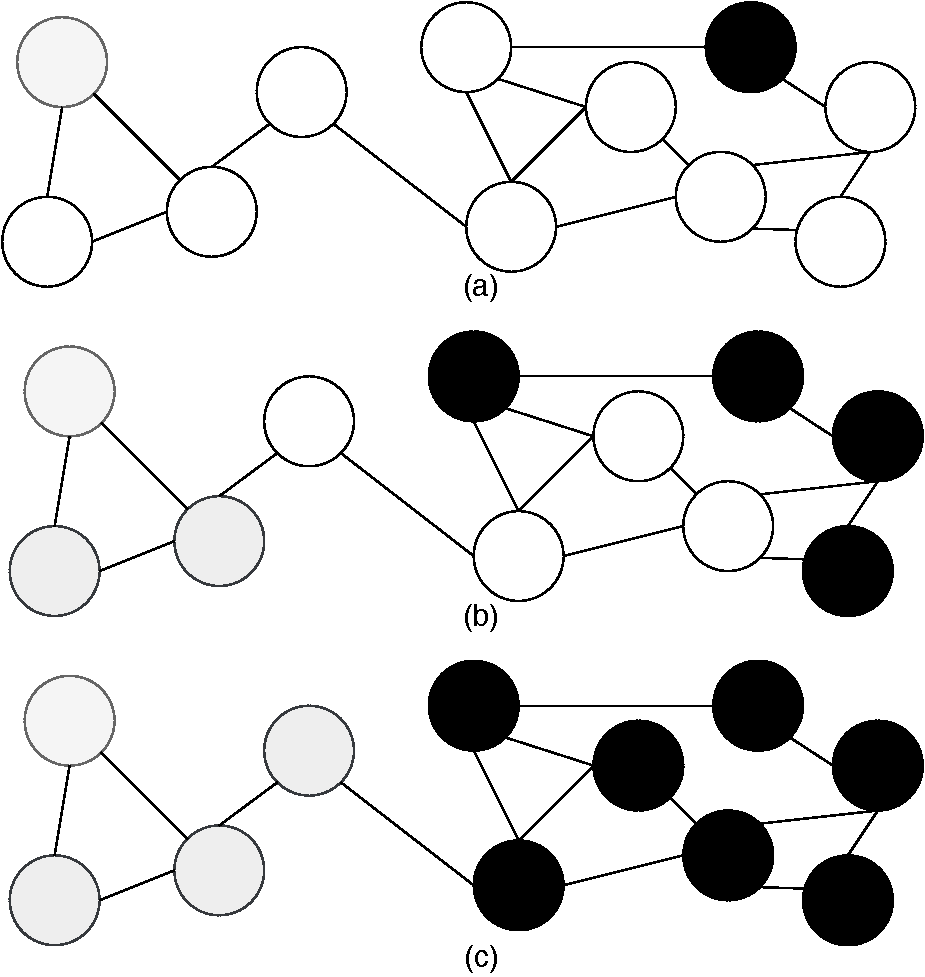
\includegraphics[scale=0.35]{figures/label_propagation.pdf}}
    \caption{(a) Step 1- Random tags have been initialized which is a sem-supervised method, (b) Step 2- In this step tags are adopted from neighbors, and (c) Step 3- Finally all nodes have been assigned tags}
    \label{fig6}
\end{figure}

This algorithm performs near-linear time as mentioned by Raghavan et al.\cite{16} which makes it a better contender among other community analysis algorithms. The time complexity is given by O($n + e$) where $n$ is nodes in a graph and $e$ is edges.

\subsubsection{Louvain Modularity}
Louvain modularity algorithm is used to identify the quality or accuracy of a community. It also helps in formation of communities in huge networks. It is a hierarchical clustering algorithm. This algorithm was developed by Blondel et al. in 2008 \cite{20}. Using modularity, it also analyses the accuracy of community formation. Blondel et al. calimed that it is an exceptional algorithm in terms of accuracy to extract communities among other community formation algorithms and gives good performance on large graphs.

The algorithm compares newly formed communities with random network based on the density of nodes in a community. It does so by assigning modularity scores to the communities. Modularity score is the measure of how well nodes are divided into communities. The figure \ref{fig7} shown below will help in understanding the working of the algorithm.

\begin{figure}[!h]
    \centerline{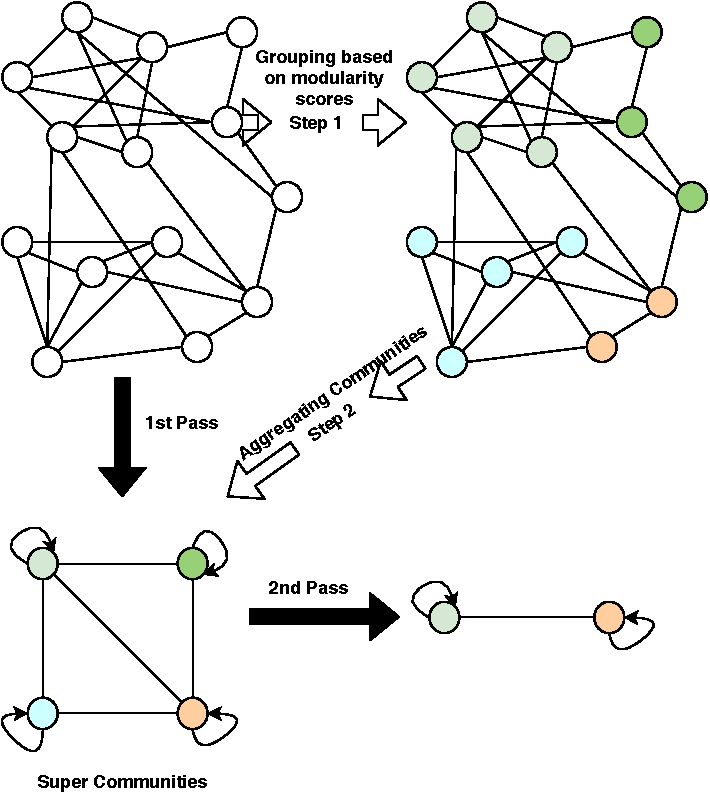
\includegraphics[scale=0.7]{figures/louvain.pdf}}
    \caption{Louvain Modularity algorithm applied on a graph. The algorithm works in two passes. First pass involves communities formation and aggregation to form super communities; second pass peforms aggregation on these communities to create new communities in the network}
    \label{fig7}
\end{figure}

Time complexity is given by O($n^2$) where $n$ is the number of nodes. This algorithm has been used for creating recommendation systems\cite{55}, extracting trends from social media\cite{56}, and understanding community structures in the human brain network\cite{57}.

\subsubsection{Node Clustering Coefficient}


\subsubsection{Average Clustering Coefficient}
\subsubsection{Bron-Kerbosch}

\subsection{Centrality Analysis}
Centrality analysis is used to identify the relevance between each node. It measures the importance of nodes. It is used to find the influence of people in a social network, used to get the most popular web page based on access, and key nodes in a network. Although this method was introduced specifically for social network analysis, it has been adopted in many other fields.

\subsubsection{Degree Centrality}
Degree centrality was proposed by Freeman in 1979\cite{25}. It is used for measuring the relationships of a node. For a directed graph, it divides the relationships into indegree and outdegree where indegree is the number of connections coming in while outdegree is the number of connections going out of the node. It shows the activity of a node. In simple terms, it states higher the number of neighbors more important the node is. This way degree centrality is used for identifying most influential accounts on Twitter or other social networking platforms. Since it just involves propagating through the network and calculates the degree(inwards and outwards connections) of each node, it is a simple method to implement. The following figure \ref{fig8} depicts a network of nodes with degree centrality algorithm applied over it.

\begin{figure}[!h]
    \centerline{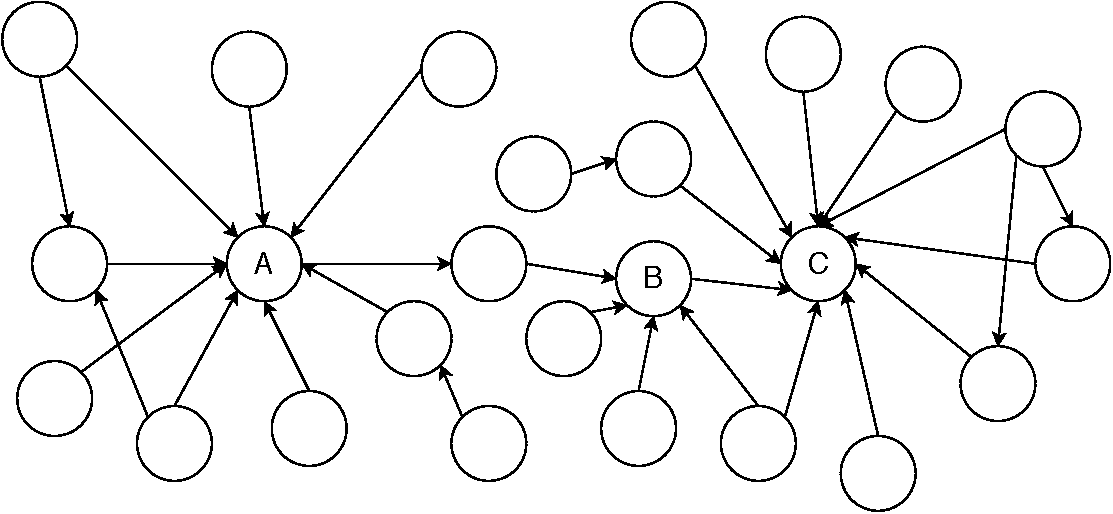
\includegraphics[scale=0.45]{figures/degree_centrality.pdf}}
    \caption{As it can be noticed in the figure, the number of inward connections in node A is 9, node B has 5, and node C has 10}
    \label{fig8}
\end{figure}

The time complexity of this algorithm thus will be O($v$) where $v$ is vertices of the graph.

\subsubsection{Eigenvector Centrality}
The eigenvector centrality method was proposed by Bonacich\cite{26}. It is the influence a node has in a network. A node is scored based on its connections with nodes with high scores. This means, a node connected to a few other nodes but these nodes have high influence, then the former node's eigenvector value will be very high. It can be inferred that connecting to a few highly influential nodes will give a boost in the eigenvector value.

When the algorithm initializes, every node starts with an equal or zero value. As the algorithm computes scores, nodes with a higher number of connections will get high scores. These high scores are then propagated to their connected nodes. The algorithm performs a few iterations until the value stabilizes. Thus generating eigenvector value for all nodes. The following figure \ref{fig9} shows nodes connected.

\begin{figure}[!h]
    \centerline{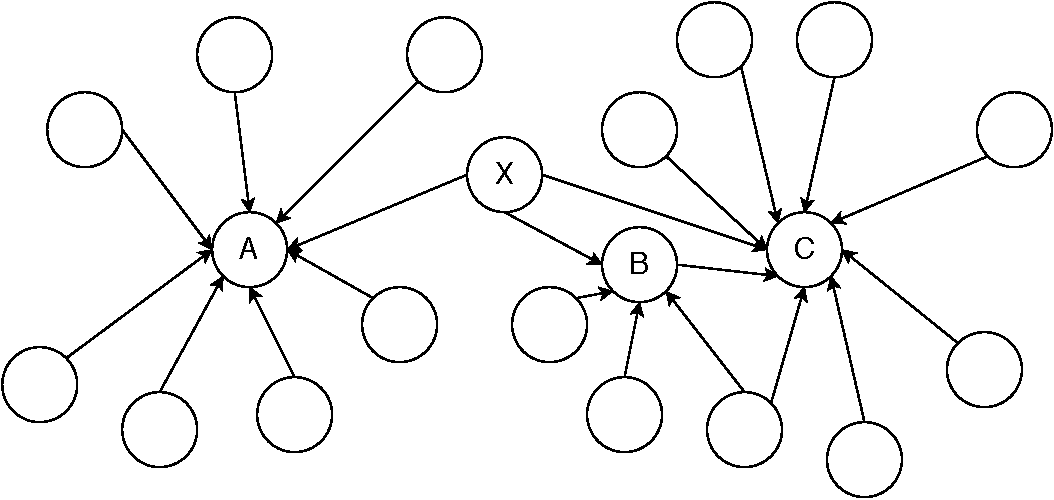
\includegraphics[scale=0.45]{figures/eigenvector_centrality.pdf}}
    \caption{Here, X has the highest eigenvector value as it is connected to the highest number of significant or high influence nodes}
    \label{fig9}
\end{figure}

\subsubsection{Katz Centrality}
\subsubsection{PageRank Centrality}
\subsubsection{Closeness Centrality}
\subsubsection{Betweenness Centrality}


\subsection{Graph Neural Networks}
\label{sec:gnn}

\section{Discussion}
\label{sec:discussion}

\section{Conclusion}
\label{sec:conclusion}

\begin{thebibliography}{9}
    \bibitem{1}“Resources - Whitepapers, Infographics \& Webinars | Domo.” [Online]. Available: https://www.domo.com/learn.
    
    \bibitem{2}C. Petrov, “Big Data Statistics 2019,” Tech Jury. [Online]. Available: https://techjury.net/stats-about/big-data-statistics
    
    \bibitem{3}“Domo Resource - Data Never Sleeps 7.0.” [Online]. Available: https://www.domo.com/learn/data-never-sleeps-7.
    
    \bibitem{4}“A Short History Of Big Data,” Datafloq. [Online]. Available: https://datafloq.com/read/big-data-history/239.
    
    \bibitem{5}E. Team, “How Netflix Uses Big Data to Drive Success,” inside BIGDATA, 20-Jan-2018.
    
    \bibitem{6}“Wikibon’s 2018 Big Data Analytics Trends and Forecast,” Wikibon Research, 28-Feb-2018. .
    
    \bibitem{7}“What is graph analytics?,” IBM Big Data \& Analytics Hub. [Online]. Available: https://www.ibmbigdatahub.com/blog/what-graph-analytics. [Accessed: 12-Dec-2019].
    
    \bibitem{8}A. Buluç and K. Madduri, “Parallel Breadth-First Search on Distributed Memory Systems,” p. 12.
    
    \bibitem{9}V. N. Rao and V. Kumar, “Parallel depth first search. Part I. Implementation,” Int J Parallel Prog, vol. 16, no. 6, pp. 479–499, Dec. 1987.
    
    \bibitem{10}M. Naumov, A. Vrielink, and M. Garland, “Parallel Depth-First Search for Directed Acyclic Graphs,” in Proceedings of the Seventh Workshop on Irregular Applications: Architectures and Algorithms - IA3’17, Denver, CO, USA, 2017, pp. 1–8.
    
    \bibitem{11}M. Kranjčević, D. Palossi, and S. Pintarelli, “Parallel Delta-Stepping Algorithm for Shared Memory Architectures,” arXiv:1604.02113 [cs], Apr. 2016.
    
    \bibitem{12}J. W. Kim, H. Choi, and S.-H. Bae, “Efficient Parallel All-Pairs Shortest Paths Algorithm for Complex Graph Analysis,” in Proceedings of the 47th International Conference on Parallel Processing Companion, New York, NY, USA, 2018, pp. 5:1–5:10.
    
    \bibitem{13}L. Fitina, J. Imbal, V. Uiari, N. Murki, and E. Goodyear, “An Application of Minimum Spanning Trees to Travel Planning,” vol. 12, p. 11, 2010.
    
    \bibitem{14}L. L. Sz, “Random Walks on Graphs: A Survey,” p. 46.
    
    \bibitem{15}M. Sharir, “A strong-connectivity algorithm and its applications in data flow analysis,” Computers \& Mathematics with Applications, vol. 7, no. 1, pp. 67–72, Jan. 1981.
    
    \bibitem{16}U. N. Raghavan, R. Albert, and S. Kumara, “Near linear time algorithm to detect community structures in large-scale networks,” Phys. Rev. E, vol. 76, no. 3, p. 036106, Sep. 2007.
    
    \bibitem{17}R. Tarjan, “Depth-First Search and Linear Graph Algorithms,” SIAM J. Comput., vol. 1, no. 2, pp. 146–160, Jun. 1972.
    
    \bibitem{18}A. Monge and C. Elkan, An Efficient Domain-Independent Algorithm for Detecting Approximately Duplicate Database Records. 1997.
    
    \bibitem{19}Y. An, J. Janssen, and E. E. Milios, “Characterizing and Mining the Citation Graph of the Computer Science Literature,” Know. Inf. Sys., vol. 6, no. 6, pp. 664–678, Nov. 2004.
    
    \bibitem{20}V. D. Blondel, J.-L. Guillaume, R. Lambiotte, and E. Lefebvre, “Fast unfolding of communities in large networks,” J. Stat. Mech., vol. 2008, no. 10, p. P10008, Oct. 2008.
    
    \bibitem{21}H. Lu, M. Halappanavar, and A. Kalyanaraman, “Parallel Heuristics for Scalable Community Detection,” arXiv:1410.1237 [physics], Oct. 2014.
    
    \bibitem{22}T. Schank and D. Wagner, “Finding, Counting and Listing All Triangles in Large Graphs, an Experimental Study,” in Experimental and Efficient Algorithms, vol. 3503, S. E. Nikoletseas, Ed. Berlin, Heidelberg: Springer Berlin Heidelberg, 2005, pp. 606–609.
    
    \bibitem{23}H. C. Johnston, “Cliques of a graph-variations on the Bron-Kerbosch algorithm,” International Journal of Computer and Information Sciences, vol. 5, no. 3, pp. 209–238, Sep. 1976.
    
    \bibitem{24}S. C. Antoro, K. A. Sugeng, and B. D. Handari, “Application of Bron-Kerbosch algorithm in graph clustering using complement matrix,” presented at the International Symposium On Current Progress In Mathematics And Sciences 2016 (ISCPMS 2016): Proceedings of the 2nd International Symposium on Current Progress in Mathematics and Sciences 2016, Depok, Jawa Barat, Indonesia, 2017, p. 030141.
    
    \bibitem{25}L. C. Freeman, “Centrality in social networks conceptual clarification,” Social Networks, vol. 1, no. 3, pp. 215–239, Jan. 1978.
    
    \bibitem{26}Phillip Bonacich Reviewed, “Power and Centrality: A Family of Measures,” American Journal of Sociology, vol. 92, no. 5, pp. 1170–1182, 1987.
    
    \bibitem{27}C. F. A. Negre et al., “Eigenvector centrality for characterization of protein allosteric pathways,” Proc Natl Acad Sci U S A, vol. 115, no. 52, pp. E12201–E12208, Dec. 2018.
    
    \bibitem{28}L. Katz, “A new status index derived from sociometric analysis,” Psychometrika, vol. 18, no. 1, pp. 39–43, Mar. 1953.
    
    \bibitem{29}L. Page, S. Brin, R. Motwani, and T. Winograd, “The PageRank Citation Ranking: Bringing Order to the Web.,” 11-Nov-1999. [Online]. Available: http://ilpubs.stanford.edu:8090/422/. [Accessed: 12-Dec-2019].
    
    \bibitem{30}G. Sabidussi, “The centrality index of a graph,” Psychometrika, vol. 31, no. 4, pp. 581–603, Dec. 1966.
    
    \bibitem{31}S. P. Borgatti, “Centrality and network flow,” Social Networks, vol. 27, no. 1, pp. 55–71, Jan. 2005.
    
    \bibitem{32}L. C. Freeman, “A Set of Measures of Centrality Based on Betweenness,” Sociometry, vol. 40, no. 1, pp. 35–41, 1977.
    
    \bibitem{33}Z. Wu, S. Pan, F. Chen, G. Long, C. Zhang, and P. S. Yu, “A Comprehensive Survey on Graph Neural Networks,” arXiv:1901.00596 [cs, stat], Dec. 2019.
    
    \bibitem{34}F. Scarselli, M. Gori, Ah Chung Tsoi, M. Hagenbuchner, and G. Monfardini, “The Graph Neural Network Model,” IEEE Trans. Neural Netw., vol. 20, no. 1, pp. 61–80, Jan. 2009.
    
    \bibitem{35}“Special Issue on Graph-based Methods for Large Scale Financial and Business Data Analysis - Call for Papers - Elsevier.” [Online]. Available: https://www.journals.elsevier.com/pattern-recognition/call-for-papers/graph-based-methods. [Accessed: 09-Dec-2019].
    
    \bibitem{36} R. K. Ghosh and G. P. Bhattacharjee, “Parallel breadth-first search algorithms for trees and graphs,” International Journal of Computer Mathematics, vol. 15, no. 1–4, pp. 255–268, Jan. 1984, doi: 10.1080/00207168408803413.

    \bibitem{37} “Parallel breadth-first search,” Wikipedia. 03-Nov-2019. [Online]. Available: https://en.wikipedia.org/wiki/Parallel{\_}breadth-first{\_}search. [Accessed: 06-Jan-2020].

    \bibitem{38} J. Freeman, “Parallel Algorithms for Depth-First Search,” Technical Reports (CIS), Oct. 1991.

    \bibitem{39} “Strongly Connected Components Algorithm Optimized,” Weiming Hu. [Online]. Available: https://weiming-hu.github.io/strongly-connected-components/. [Accessed: 06-Jan-2020].

    \bibitem{40} “Kosaraju’s algorithm,” Wikipedia. 07-Mar-2019.  Available: https://en.wikipedia.org/wiki/Kosaraju's{\_}algorithm. [Accessed: 06-Jan-2020].

    \bibitem{41} J. Bang-Jensen and G. Z. Gutin, Digraphs: Theory, Algorithms and Applications, 2nd ed. London: Springer-Verlag, 2009.

    \bibitem{42} A. Shimbel, “Structural parameters of communication networks,” Bulletin of Mathematical Biophysics, vol. 15, no. 4, pp. 501–507, Dec. 1953, doi: 10.1007/BF02476438.

    \bibitem{43} L. Roditty and U. Zwick, “On Dynamic Shortest Paths Problems,” Algorithmica, vol. 61, no. 2, pp. 389–401, Oct. 2011, doi: 10.1007/s00453-010-9401-5.

    \bibitem{44} S. Pettie, “A new approach to all-pairs shortest paths on real-weighted graphs,” Theoretical Computer Science, vol. 312, no. 1, pp. 47–74, Jan. 2004, doi: 10.1016/S0304-3975(03)00402-X.

    \bibitem{45} W. Peng, X. Hu, F. Zhao, and J. Su, “A Fast Algorithm to Find All-Pairs Shortest Paths in Complex Networks,” Procedia Computer Science, vol. 9, pp. 557–566, 2012, doi: 10.1016/j.procs.2012.04.060.

    \bibitem{46} T. M. Chan, “All-Pairs Shortest Paths with Real Weights in O(n 3/log n) Time,” Algorithmica, vol. 50, no. 2, pp. 236–243, Feb. 2008, doi: 10.1007/s00453-007-9062-1.

    \bibitem{47} J. Nešetřil, E. Milková, and H. Nešetřilová, “Otakar Borůvka on minimum spanning tree problem Translation of both the 1926 papers, comments, history,” Discrete Mathematics, vol. 233, no. 1, pp. 3–36, Apr. 2001, doi: 10.1016/S0012-365X(00)00224-7.

    \bibitem{48} V. Jarník, “O jistém problému minimálním. (Z dopisu panu O. Borůvkovi).”
    
    \bibitem{49} BSTJ 36: 6. November 1957: Shortest Connection Networks And Some Generalizations. (Prim, R.C.). 1957.

    \bibitem{50} E. Spada et al., “Use of the Minimum Spanning Tree Model for Molecular Epidemiological Investigation of a Nosocomial Outbreak of Hepatitis C Virus Infection,” J Clin Microbiol, vol. 42, no. 9, pp. 4230–4236, Sep. 2004, doi: 10.1128/JCM.42.9.4230-4236.2004.

    \bibitem{51} E. Codling, M. Plank, and S. Benhamou, “Random walks in biology,” Journal of the Royal Society, Interface / the Royal Society, vol. 5, pp. 813–34, Sep. 2008, doi: 10.1098/rsif.2008.0014.
    
    \bibitem{52} “The Random Walk Theory And Stock Prices: Evidence From Johannesburg Stock Exchange.” [Online]. Available: https://www.researchgate.net/publication/297750180{\_}The{\_}Random{\_}Walk{\_}Theory{\_}And{\_}Stock{\_}Prices{\_}Evidence{\_}From{\_}Johannesburg{\_}Stock{\_}Exchange. [Accessed: 30-Jan-2020].

    \bibitem{53} N. Masuda, M. A. Porter, and R. Lambiotte, “Random walks and diffusion on networks,” Physics Reports, vol. 716–717, pp. 1–58, Nov. 2017, doi: 10.1016/j.physrep.2017.07.007.
    
    \bibitem{54} D. Mack, “Review prediction with Neo4j and TensorFlow,” Medium, 25-Apr-2018. [Online]. Available: https://medium.com/octavian-ai/review-prediction-with-neo4j-and-tensorflow-1cd33996632a. [Accessed: 30-Jan-2020].
    
    \bibitem{55} V. Sundaresan, I. Hsu, and D. Chang, “Subreddit Recommendations within Reddit Communities,” p. 10.

    \bibitem{56} G. S. Kido, R. A. Igawa, and S. Barbon Jr., “Topic Modeling based on Louvain method in Online Social Networks,” in Anais do Simpósio Brasileiro de Sistemas de Informação (SBSI), 2016, pp. 353–360, doi: 10.5753/sbsi.2016.5982.
    
    \bibitem{57} D. Meunier, R. Lambiotte, A. Fornito, K. D. Ersche, and E. T. Bullmore, “Hierarchical Modularity in Human Brain Functional Networks,” Front Neuroinformatics, vol. 3, Oct. 2009, doi: 10.3389/neuro.11.037.2009.

\end{thebibliography}


\end{document}